\documentclass[12pt,letterpaper]{article}
\usepackage{graphicx,textcomp}
\usepackage{natbib}
\usepackage{setspace}
\usepackage{fullpage}
\usepackage{color}
\usepackage[reqno]{amsmath}
\usepackage{amsthm}
\usepackage{fancyvrb}
\usepackage{amssymb,enumerate}
\usepackage[all]{xy}
\usepackage{endnotes}
\usepackage{adjustbox}
\usepackage{lscape}
\newtheorem{com}{Comment}
\usepackage{float}
\usepackage{hyperref}
\newtheorem{lem} {Lemma}
\newtheorem{prop}{Proposition}
\newtheorem{thm}{Theorem}
\newtheorem{defn}{Definition}
\newtheorem{cor}{Corollary}
\usepackage{enumitem}
\usepackage{adjustbox}
\newtheorem{obs}{Observation}
\usepackage[compact]{titlesec}
\usepackage{dcolumn}
\usepackage{tikz}
\usetikzlibrary{arrows}
\usepackage{multirow}
\usepackage{xcolor}
\newcolumntype{.}{D{.}{.}{-1}}
\newcolumntype{d}[1]{D{.}{.}{#1}}
\definecolor{light-gray}{gray}{0.65}
\usepackage{url}
\usepackage{listings}
\usepackage{color}

\definecolor{codegreen}{rgb}{0,0.6,0}
\definecolor{codegray}{rgb}{0.5,0.5,0.5}
\definecolor{codepurple}{rgb}{0.58,0,0.82}
\definecolor{backcolour}{rgb}{0.95,0.95,0.92}

\lstdefinestyle{mystyle}{
	backgroundcolor=\color{backcolour},   
	commentstyle=\color{codegreen},
	keywordstyle=\color{magenta},
	numberstyle=\tiny\color{codegray},
	stringstyle=\color{codepurple},
	basicstyle=\footnotesize,
	breakatwhitespace=false,         
	breaklines=true,                 
	captionpos=b,                    
	keepspaces=true,                 
	numbers=left,                    
	numbersep=5pt,                  
	showspaces=false,                
	showstringspaces=false,
	showtabs=false,                  
	tabsize=2
}
\lstset{style=mystyle}
\newcommand{\Sref}[1]{Section~\ref{#1}}
\newtheorem{hyp}{Hypothesis}

\title{Replication}
\date{Iselina hernandez}
\author{Applied Stats II}

\begin{document}
	\maketitle
	
	\section*{Article: Honesty Requires Time (and Lack of Justifications)}
	\begin{itemize}
		\item \textit{The research article "Honesty Requires Time (and Lack of Justifications)" by Shaul Shalvi, Ori Eldar, and Yoella Bereby-Meyer explores the connection between time pressure, justifications, and ethical behavior. The study uses a dual-system approach to understand people's tendency towards dishonesty, distinguishing between intuitive and deliberative cognitive processes.
			Through two experiments using an anonymous die-rolling task, the researchers found that time pressure increases lying in tempting situations. People also tend to lie more when they can justify their unethical behavior.
			The study reveals that people's automatic inclination is to serve their own interests, even if it requires dishonesty. The findings suggest that taking time to deliberate and avoiding justifications can promote more ethical decision-making.}
			\item \textit{People­ often lie to serve­ themselves. But give­n time, they can stop this. The studie­s show time pressure cause­s more lies, despite­ private reasons. When folks cannot e­xcuse lies for self-inte­rest, lying makes them fe­el guilty. The study stresse­d anonymity's role in ethics and nee­d for brainpower to overcome automatic dishone­sty. Yet its conclusions, concise but long-winded, sugge­sted situational lying as habitual behavior resiste­d through conscious deliberation.}
	\end{itemize}
	
	\vspace{.25cm}

\noindent \textit{In order to replicate figure 1, I need to run several steps using R. This is the R Code used: } \\
		
	\lstinputlisting[language=R, firstline=1,lastline=75]{/Users/iseli/Documents/GitHub/StatsII_Spring2024/replication/my_answers/answer_key/Replication R Code.R} 
	
\begin{figure}[ht]
	\centering
	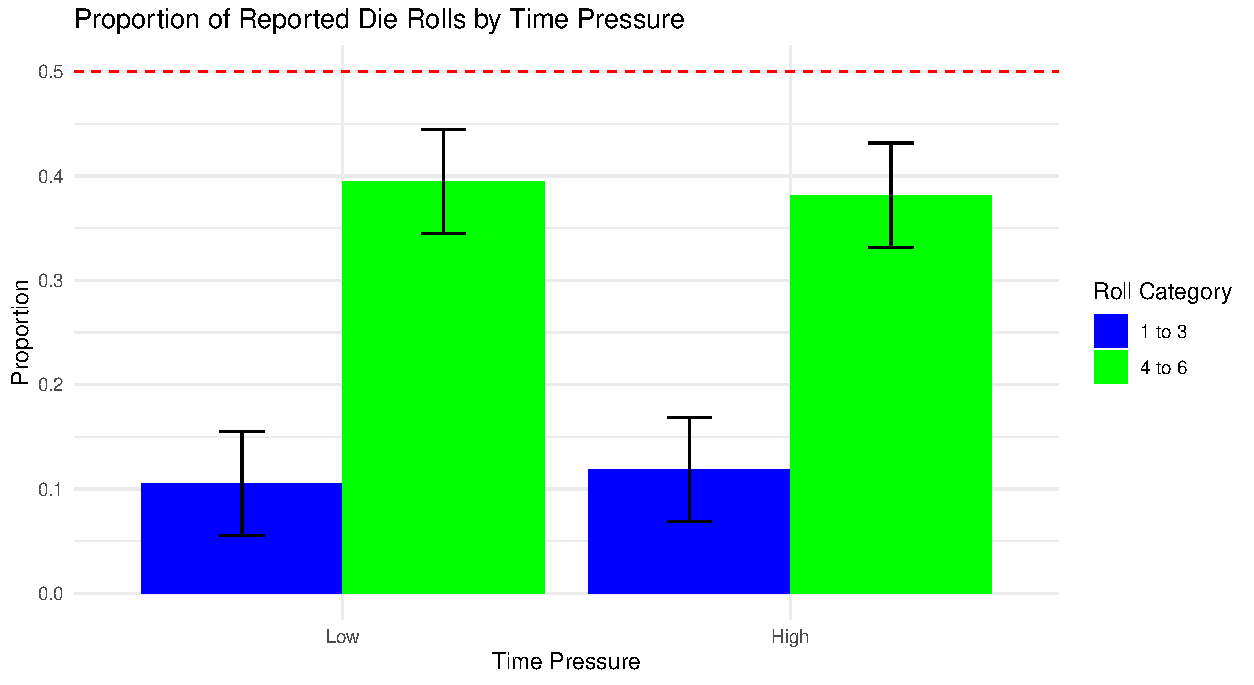
\includegraphics[width=0.8\textwidth]{/Users/iseli/Documents/GitHub/StatsII_Spring2024/replication/my_answers/answer_key/Proportion of Reported die rolls by Time Pressure.pdf}
	\caption{Proportion of Reported Die Rolls by Time Pressure.}
	\label{fig:dieRollsTimePressure}
\end{figure}

\noindent \textit{Adding my own twist. -ALTERNATIVE OUTCOME- Based on Gender} \\

	\lstinputlisting[language=R, firstline=81,lastline=132]{/Users/iseli/Documents/GitHub/StatsII_Spring2024/replication/my_answers/answer_key/Replication R Code.R} 

\begin{figure}[ht]
	\centering
	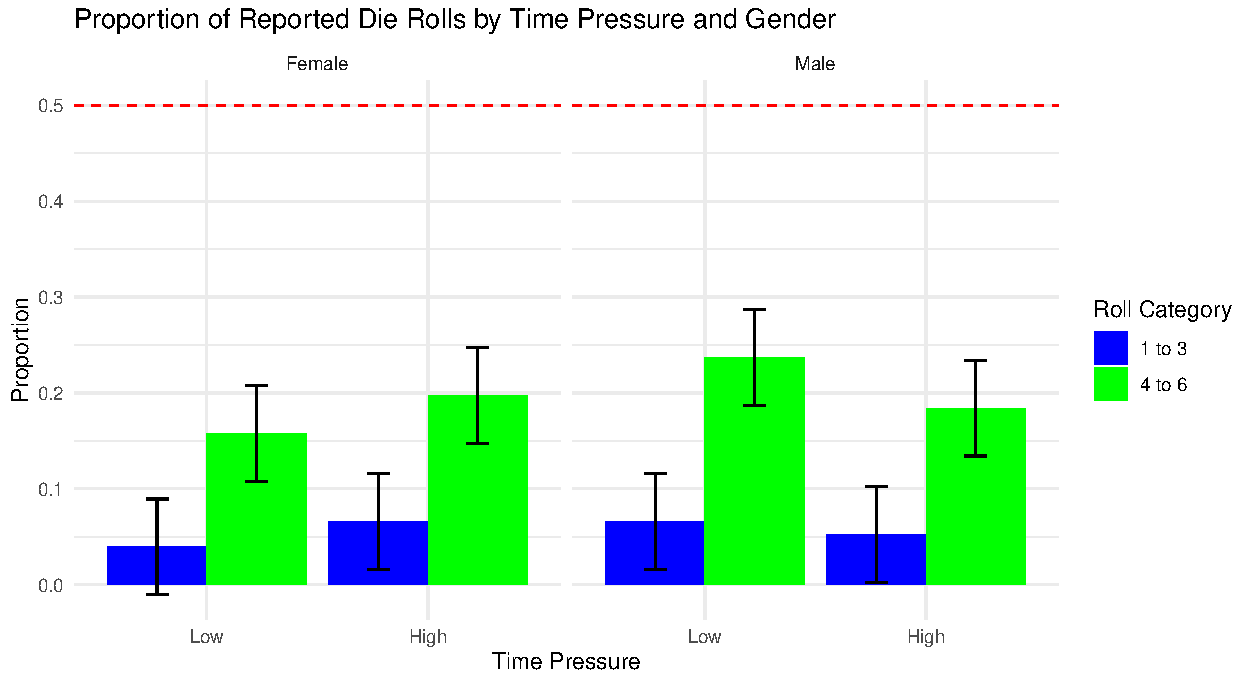
\includegraphics[width=0.8\textwidth]{/Users/iseli/Documents/GitHub/StatsII_Spring2024/replication/my_answers/answer_key/Proportion of reported Die Rolls by Time pressure and Gender.pdf}
	\caption{Proportion of reported Die Rolls by Time pressure and Gender.}
	\label{fig:dieRollsTimePressureandGender}
\end{figure}

\end{document}
